\chapter{Approach}
\index{Approach%
@\emph{Approach}}%
\label{ch:approach}

This chapter discusses the architectural approach behind Speakur\index{Speakur}, 
a social discussion plugin for the desktop and mobile web based on Web Components\index{Web Components} and the Polymer\index{Polymer} framework.
Web authors can use Speakur to easily add a comment section to their articles or blog posts.
Visitors can leave feedback about the article and engage in discussion with each other.
Discussions are grouped into topics or `threads', and within these threads, users can reply to the main article or to each other.

\section{Functionality}
Speakur\index{Speakur} 
is a Custom Element\index{Custom Elements} 
(\tcode{<speakur-discussion>}\index{<speakur-discussion>}) 
that provides an embeddable discussion forum or comment hosting service for a blog, web page or other web application.
Examples of Speakur's user interface\index{user interface (UI)} can be found in Figures~\ref{f:demo1} and~\ref{f:lang}.
Placing Speakur inside a web resource is very straightforward.
As shown in Listing~\ref{l:example1},
and in section \ref{publishing} below,
you simply place the \tcode{<speakur-discussion>}\index{<speakur-discussion>}
 element in your page's HTML\index{HTML} at the desired spot.
This requires two supporting steps detailed in section~\ref{publishing}:
\begin{enumerate}
\item loading the Web Components\index{Web Components} polyfill\index{polyfill} script
\item importing the \tcode{<speakur-discussion>}\index{<speakur-discussion>} element.
\end{enumerate}

Once an author imports the element and places it on their page, that site now has an integrated discussion forum for desktop and mobile\index{mobile} users. 
All forum data including user profiles and comment text is stored in an online cloud database called Firebase~\cite{firebasecontributors2015}\index{Firebase}.
The messy details of structuring a discussion forum are abstracted\index{abstraction} away from the web page author.

\tcode{<speakur-discussion>}\index{<speakur-discussion>} presents a simplified interface (API)\index{API} to users.
There are only a few options available including the URL of the Firebase instance and the thread target URL or \tcode{href}\index{href}.
If you do not provide your own Firebase\index{Firebase} URL, by default, my resource-limited database is used instead.
Therefore serious users will wish to use their own Firebase account with their own database.

In addition to basic commenting features, Speakur\index{Speakur} offers the ability to vote comments up or down, custom profiles, 
the ability to leave comments in Markdown\index{Markdown} syntax~\cite{githubcontributors2015} with syntax highlighting\index{syntax highlighting} for common programming languages, 
and (rough) user interface translations  or localizations\index{localization}\index{internationalization} 
into 15 languages as shown in Figure~\ref{f:lang}.

\begin{figure}[htb]
\centering
 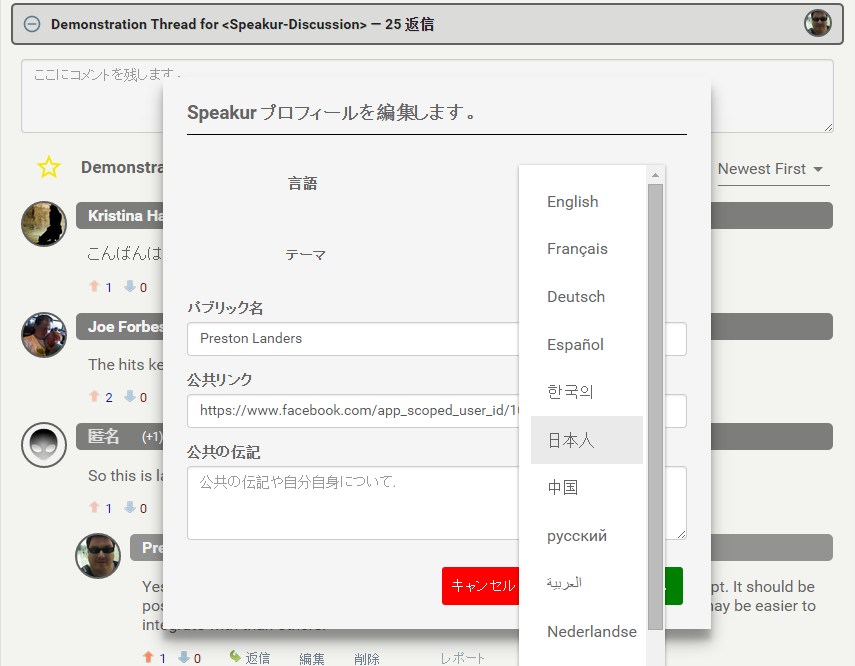
\includegraphics[width=\textwidth]{images/screenshot_20150320_1923_lang.png}
\caption{Speakur's interface language\index{internationalization} updates instantly upon selection.}
\label{f:lang}
\end{figure}

From a technical perspective, one of the more interesting features in Speakur\index{Speakur} is the use of Polymer's\index{Polymer} data-bound templates\index{data-bound template}, also known as Model-Driven Views\index{Model-Driven View}, 
to allow components to automatically reflect changes in far-flung areas of the application.
Also, Firebase's\index{Firebase} event notification\index{event notification} architecture allows all web clients to instantly and transparently reflect any changes in another remote client.
Another example of the power of data-bound templates is that all of the user-visible text in the application immediately updates as soon as the user changes his or her locale preference in the dialog in Figure~\ref{f:lang}.

\section{Architecture overview}
It has been said that ``any problem in computer science can be solved with another layer of indirection\index{indirection}'' (usually attributed to Wheeler).
The key to understanding a software package is learning its architecture\index{architecture},
which is really a map of these layers of indirection\index{indirection} and abstraction\index{abstraction}.
Roy Fielding, the author of the influential REST\index{REST} web architecture\index{architecture}, described a software architecture as:

\begin{quote}
\dots an abstraction of the run-time elements of a software system during some phase of its operation. A system may be composed of many levels of abstraction and many phases of operation, each with its own software architecture.

At the heart of software architecture is the principle of abstraction: hiding some of the details of a system through encapsulation\index{encapsulation} in order to better identify and sustain its properties. A complex system will contain many levels of abstraction, each with its own architecture~\cite{fielding2000}.
\end{quote}

The architecture for Speakur\index{Speakur} is based on client-side (browser) JavaScript\index{JavaScript} code and HTML\index{HTML} layout following the Web Components\index{Web Components} design principles listed in section~\ref{sec:wcprinciples} below. 
There is no dedicated server component except for the Firebase\index{Firebase} cloud database service~\cite{firebasecontributors2015}.
Speakur is built entirely from plain HTML, JS and CSS\index{CSS} files that can be served from a content delivery network (CDN)\index{content delivery network (CDN)} 
such as \tcode{github.io}\index{GitHub} or your own server~\cite{landers2015-d}.
This low-overhead design allows Speakur\index{Speakur} to be used on your own website without actually `installing' any software;
just load Speakur directly from \tcode{github.io} with an HTML \textit{import}
and then insert a tiny bit of HTML markup into your document~\cite{landers2015-d}.
This helps fulfill the ease of use requirements 
\#\ref{motive:abstraction} and \#\ref{motive:cors}
in section~\ref{motivations}.

Most of the user interface\index{user interface (UI)} elements in Speakur\index{Speakur} 
--- things like dropdown menus and dialogs as well as invisible functional components like expand/collapse elements  
--- are implemented with Polymer's\index{Polymer} Core\index{Core Elements} and Paper\index{Paper Elements} custom element libraries.
Speakur presents a simple API through \tcode{<speakur-discussion>}\index{<speakur-discussion>},
but internally it consists of a number of internal abstraction layers or custom elements.
In turn, these internal layers consist of still more focused layers, other Polymer\index{Polymer} components, 
simple HTML templates, 
and wrappers around external JavaScript\index{JavaScript} libraries 
like \tcode{moment.js}\index{moment.js library}.
These internal layers are described in section~\ref{sec:layout}.

As previously mentioned, in order to make the 
\tcode{<speakur-discussion>}\index{<speakur-discussion>} element available for use, 
you must first load the Web Components polyfill\index{polyfill} and then \textit{import} the Speakur element, 
either from \tcode{github.io} or your own server.
I recommend that you create your own Firebase\index{Firebase} instance for data security and resource limitation reasons, but even this is not required. 
The author's demonstration database is used by default.

Security\index{security} for web clients engaging in data manipulation 
(i.e, posting, editing or deleting comments) 
is handled entirely through the Firebase\index{Firebase} authentication\index{authentication} 
and data security\index{security} rules described below.
The simplicity of this arrangement makes it easier to fit Speakur\index{Speakur} into almost any web application architecture\index{architecture}.

\section{Responsive design}
\label{bg:mobile}
Although native apps are frequently preferred by mobile users and developers, 
the mobile web remains an important development platform for the same reason that 
desktop web apps continue to live alongside native desktop apps; 
web apps typically do not require installing anything to the device, are always up-to-date, and have a lower barrier to entry overall for users and developers.
Because Speakur\index{Speakur} is not a standalone application but rather a plug-in designed to be embedded into other web pages or apps, 
the full document is not under its control.
This can affect the mobile\index{mobile} user experience\index{user experience (UX)},
but within these limits, Speakur strives to present a responsive\index{responsive design} interface to different screen sizes.

\begin{figure}[htb]
\centering
 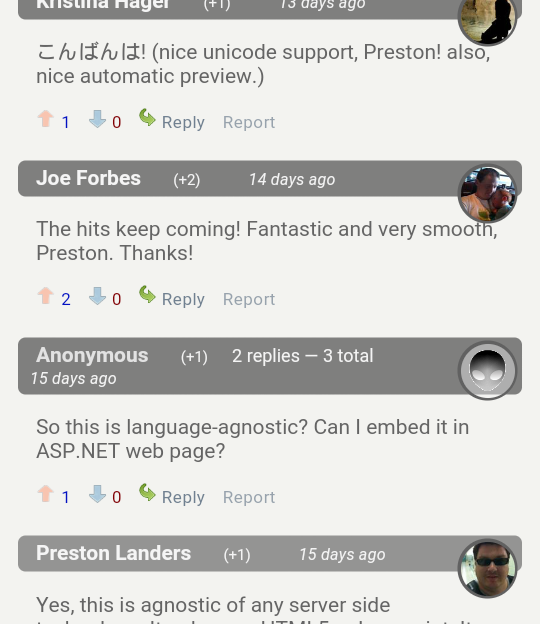
\includegraphics[width=3in]{images/mobile2.png}
\caption{Speakur thread on a mobile phone.}
\label{f:mobile1}
\end{figure}

The two main techniques used in Speakur\index{Speakur} for responsive design are CSS\index{CSS} flexible (flex)\index{Flex} boxes~\cite{mozillacontributors2015} 
and CSS \tcode{@media}\index{@media} rules that apply varied styles to different screen sizes. 
In addition, Speakur's JavaScript\index{JavaScript} code exposes a \tcode{smallScreen} flag to the HTML templates\index{HTML!templates} that can trigger layout adjustments, 
such as moving the user photo to a different location.

The desktop version in Figure~\ref{f:demo1} shows the user photo to the left of the main post area, 
but the mobile version in Figure~\ref{f:mobile1} above shows how the user photo is moved to the right side of the post header. 
A CSS\index{CSS} \tcode{@media}\index{@media} rule for small screens disables the indentation of replies shown at the bottom of Figure~\ref{f:demo1}. 
The extensive use of CSS flex\index{Flex} box attributes ensures that structural elements like headers and toolbars automatically adjust their layout to available space~\cite{polymercontributors2015-d}. 
This will be described in more detail in section~\ref{sec:responsive}.

\section{Polymer and Web Components}
As described in Chapter~\ref{ch:background}, 
Web Components\index{Web Components} are a 
W3C\index{W3C} initiative 
to expose certain native browser features in a public, standardized way. 
Polymer\index{Polymer} is a 
Google\index{Google} 
web framework built from the ground up around Web Components.
Polymer also provides the crucial 
polyfill\index{polyfill} library 
that is required for Web Component features to work on most current browsers.

In general, Speakur tries to adhere to the core principles laid out by the 
Web Components\index{Web Components} developers 
for general purpose components. 
It's worth quoting those here in full, 
because they are applicable to software engineering\index{software engineering} in general. They are:
\label{sec:wcprinciples}
\begin{quote}
\begin{enumerate}
\item Address a common need.\label{wcp:commonneed}
\item Do one job really well.\label{wcp:onejob}
\item Work predictably in a wide variety of circumstances.\label{wcp:predicatable}
\item Be useful right out of the box.\label{wcp:useful}
\item Be composable.\label{wcp:composable}
\item Be styleable.\label{wcp:stylable}
\item Be extensible.\label{wcp:extensible}
\item Think small.\label{wcp:thinksmall}
\item Adapt to the user and device.\label{wcp:adaptable}
\item Deliver the key benefit to HTML authors, not just coders~\label{wcp:htmlauthors}\cite{webcomponentscontributors2014}.
\end{enumerate}
\end{quote}

% Explain how I follow those guidelines... [TODO]
% Will be explained in ch 4 and 5, should I mention that here? probably not

The Polymer project provides two (optional) libraries of Custom Elements\index{Custom Elements} for use in your own projects. 
\textbf{Core Elements}\index{Core Elements} includes both user interface\index{user interface (UI)}
widgets and invisible functional elements.
Core Elements are minimally styled and can be used directly, 
but they are also used as `base classes' for 
\textbf{Paper Elements}\index{Paper Elements}, 
which implement the so-called `Material Design'\index{Material Design} look and feel (design language) used by apps for Google's\index{Google} Android\index{Android} mobile\index{mobile} operating system~\cite{imura2015}.
Speakur's\index{Speakur} layout is composed of native HTML5 elements, 
Core and Paper Elements, 
and Speakur's own custom elements that are used to abstract\index{abstraction} internal details.

\section{Data store and synchronization}
All persistent data in Speakur is stored in a cloud database\index{database} called Firebase~\cite{firebasecontributors2015}\index{Firebase}.
Anyone who wants to use Speakur\index{Speakur} can register for a free account on \tcode{firebase.com} and create a database instance to hold Speakur data.
No other server component is required.
Firebase is a NoSQL\index{NoSQL}-style key-value data store of the kind that has been popularized
with the growth of 
Node.js\index{Node.js}, a server-side JavaScript\index{JavaScript} environment,
and the MongoDB\index{MongoDB} NoSQL\index{NoSQL} database\index{database}~\cite{dickey2014}.

Firebase\index{Firebase} provides WebSockets\index{WebSockets}-based event notification\index{event notification} and synchronization 
as well as a security rule description format based on 
JSON\index{JSON}\footnote{JavaScript Object Notation (JSON)\index{JSON} is a popular data format because it's easily human-readable, 
but its free-form structure compared to XML\index{XML} can be both a blessing and a curse.  
It mirrors the syntax for writing data structure literals in the JavaScript\index{JavaScript} language.} 
for securing\index{security} and validating user actions.
The use of Firebase as the only server component allows for easy deployment\index{deployment} of Speakur with minimal dependencies, helping to adhere to the principles of ``think small'' and ``be useful right out of the box'' from above.
%Although Speakur's Firebase library uses the WebSockets protocol for data transfer and network event notification, 
%Firebase also provides a RESTful programming interface that uses the standard HTTP protocol.

\subsection{RESTful API}
Firebase\index{Firebase} can be used by itself as the sole provider of data services to an application, as Speakur does, or else it can be used as an auxiliary to other services or REST\index{REST} APIs\index{API}.
One of the key architectural benefits of using Firebase, 
besides its ease of deployment, 
is that its data binding and event notification\index{event notification} system allows for 
applications to respond to changes in real-time while remaining performant.

Firebase\index{Firebase} itself provides a REST\index{REST} API\index{API} for data access by programs like Speakur.
The term REST or RESTful is sometimes misunderstood,
but in Roy Fielding's original 2000 Ph.D. thesis, 
REST\index{REST} refers to transferring \textit{representations} of application state and using hypertext as the engine of 
application state\index{HATEOAS}\footnote{Known under the somewhat awkward acronym of HATEOAS\index{HATEOAS}.}~\cite{fielding2000}.
Specifically, `objects' of whatever type are represented as interlinked hypertext \textbf{\textit{resources}} that are operated on by standard HTTP verbs\index{HTTP!verbs} such as \tcode{PUT}\index{HTTP!PUT} and \tcode{DELETE}\index{HTTP!DELETE}.
For example, in a Speakur\index{Speakur} thread, a particular user comment (a post) is an abstract \textit{resource} located at the following uniform resource locator (URL):

\tcode{https://YOUR-DB.firebaseio.com/posts/\$ParentId/\$PostId}

%\tcode{/posts/\$ParentId/\$PostId}

where \tcode{\$PostId} is an identifier (id) for the post itself, and \tcode{\$ParentId} is the id of the post this is a reply to, 
which could be the top-level post (thread id.) 
In order to delete this post, one would issue an HTTP\index{HTTP} request to this URL with the \tcode{DELETE}\index{HTTP!DELETE} verb, as in this \tcode{bash} shell script snippet:

\begin{lstlisting}[language=bash,caption=
{Deleting a post with the REST API.},label=l:rest_delete,captionpos=below]
set DATABASE="https://my-firebase.firebaseio.com"
set POST="fake_post_id"  # the post to delete
set PARENT="parent_post_or_thread_id"

curl --request DELETE $DATABASE/posts/$PARENT/$POST
\end{lstlisting}
\index{curl}\index{HTTP!DELETE}

Of course, the server would be expected to check your authorization to delete this resource.
Viewing (reading) the post is done with a simple \tcode{GET}\index{HTTP!GET} request.
Creating a brand new post can be done with \tcode{PUT}\index{HTTP!PUT}.
Updating an existing post's text is done with the \tcode{POST}\index{HTTP!POST} verb.
By default, the resources are \textit{represented} as JSON\index{JSON} encoded data, 
but a client can request an alternative representation such as XML\index{XML}.
The storage format for the resource `at rest' inside the server database is irrelevant from the API\index{API} perspective.

Areas where typical web APIs\index{API} fall short of being truly ``REST-ful''\index{REST} include:
\begin{enumerate}
\item Treating URLs as endpoints for remote procedure calls (RPC\index{RPC}) instead of hypertext resources that are interlinked in exactly the same way a website is like a tree that starts from the home page and links to various resources.
\item Not closely following HTTP semantics, especially using HTTP verbs\index{HTTP!verbs} inappropriately like using \tcode{POST}\index{HTTP!POST} for all actions including deletion.
\item Not using content related HTTP headers\index{HTTP!headers} appropriately for data representations and API\index{API} versioning\index{versioning}~\cite{steveklabnik2011}.
\end{enumerate}

The Firebase\index{Firebase} API\index{API} follows typical RESTful\index{REST} patterns in data access, allowing the database\index{database} 
and its metadata\index{metadata} to be addressed as a set of linked HTTP resources starting from a single root.
In addition, Firebase client libraries use WebSockets\index{WebSockets}, 
a lower-level TCP/IP\index{TCP/IP} protocol, 
to perform event notification\index{event notification} and distributed synchronization without the overhead of polling or high-overhead HTTP 1.1\index{HTTP} requests.
WebSockets\index{WebSockets} are used to enhance performance but all of the data in Firebase\index{Firebase} 
(and hence, in Speakur\index{Speakur}) 
is accessible from the RESTful\index{REST} HTTP API\index{API} outside of a WebSocket\index{WebSockets}.

\subsection{WebSockets}
\label{sec:websockets}
The WebSockets\index{WebSockets} protocol, formally known as RFC 6455\index{RFC 6455}, 
is a TCP/IP\index{TCP/IP} protocol that can be used alongside HTTP\index{HTTP} for persistent data connections between web clients and servers~\cite{mozillacontributors2015-a}.
Its primary purpose is to avoid the overhead of having the client initiate a new HTTP connection to check on the status of something on the server, also known as polling\index{polling}.
Aside from the fact that an HTTP\index{HTTP} connection can be `upgraded' (protocol switched) to WebSockets,
there is no direct connection or dependency between HTTP and WebSockets.
They can be used independently.

Firebase\index{Firebase} uses WebSockets\index{WebSockets} rather than traditional high-overhead HTTP\index{HTTP} requests to move data back and forth to the client.
This always-on connection allows for sending nearly instant event notifications\index{event notification} to all currently active clients with minimal overhead.
In practice, this allows the application to update its state in real-time as different users read and write values the database.
The Firebase client library `subscribes' to an area of interest in the database, such as the replies to a particular thread.
It then receives notifications when these areas change and so it can update the local representation as appropriate.

\section{Security}
\label{sec:arch_security}
Because Speakur\index{Speakur} relies entirely on Firebase\index{Firebase} for data persistence, its security\index{security} model is tied heavily to Firebase capabilities. 
All Speakur code runs inside the client's web browser including the small `admin' mode.
The security architecture\index{architecture} of the web is for the most part about protecting the \textit{user} from malicious servers (and other users), not protecting the \textit{server} from the user.
It is assumed that servers protect themselves from unauthorized actions.
Because Speakur\index{Speakur} has no `server' as such, 
other than the Firebase\index{Firebase} cloud service,
that means the security mechanisms that do things like prevent users from deleting each other's posts 
must be implemented entirely within Firebase security rules.
This is discussed in more detail in section~\ref{sec:security}.

Firebase implements the two major categories of access control: authentication\index{authentication} and 
authorization\index{authorization}. 
Authentication (sometimes abbreviated \textit{authn}) answers the question ``who are you?'' 
while authorization (\textit{authz}) asks ``what are you allowed to see and do?''~\cite{stallings2011}.
Confidentiality of in-transit data is handled with Transport Layer Security (TLS)\index{transport layer security (TLS)}, 
better known as the secure socket layer (SSL)\index{secure socket layer (SSL)} or HTTPS\index{HTTP!HTTPS}.


\subsection{Authentication}

Speakur's authentication\index{authentication} and sign-in system is handled through Firebase\index{Firebase}, 
specifically Google\index{Google} and Facebook\index{Facebook} OAuth\index{OAuth} single-sign on (SSO)\index{single sign-on (SSO)}.
Users can sign into a Speakur discussion thread, and hence Firebase, through their Facebook or Google identity.
Firebase\index{Firebase} supports other authorization schemes, including account registration (``simple password''), Twitter\index{Twitter} and GitHub\index{GitHub} identities.
Site owners who use Speakur can also designate certain threads to allow anonymous commenting.

Every user who registers within a Speakur\index{Speakur} instance by signing in with one of those identity providers gets a unique identifier --- the \tcode{uid} or user ID. 
This \tcode{uid} is used extensively in the database to refer to the user, including in the security (authorization\index{authorization}) rules that are external to the actual database (i.e, security metadata\index{metadata}.) 
Thread owners also have the option of allowing anonymous posts by users who are not signed in.

\subsection{Authorization}
Authorization\index{authorization} security\index{security} rules determine what level of access a user has within the system and what they are allowed to do or see.
Speakur's\index{Speakur} security\index{security} rules are described in more detail in section~\ref{sec:security}.
The set of security rules for a Speakur database is contained in a JSON\index{JSON} encoded file that contains expressions that determined whether a given database read or write (change) is allowed. 
For example, Speakur has defined security rules which prohibit anyone from editing or deleting an existing post unless they are the original post author or an authorized administrator.
Here is an excerpt for the \tcode{posts} resource from the security rules file:

\begin{changemargin}{-0.5cm}{-1cm}
\begin{lstlisting}[language=JavaScript,caption=
{Security rules for the \tcode{posts} table (user messages).},label=l:sec_rule1,captionpos=below]
"posts": {
  ".read": true, // anyone can read posts
  ".write": false,  // deny modification by default
  "$parentId": {
    "$childId": {
      // must be admin or post owner to modify a post.
      ".write": "data.exists() ? ( auth.uid === data.child('author').child('uid').val() || root.child('admins').child(auth.uid).child('scope').val() === '*' ) : true",
      // validate structure of new posts
      ".validate": "newData.hasChildren(['threadId', 'text', 'author']) && newData.child('timestamp').val() > 1"
    }
  }
}
\end{lstlisting}
\end{changemargin}

This rule structure is dictated by the architecture\index{architecture} of Firebase\index{Firebase}.
This setup has certain pros and cons that can be seen from Listing~\ref{l:sec_rule1}. 
On one hand, it's logically designed and the expressions provide a powerful and fairly comprehensive way to specify the 
security\index{security} and authorization\index{authorization} logic for your database.
On the other hand, non-trivial rule expressions can get awkwardly long and in complex cases can devolve into a maze of nested ternary operators.
Having one big file with all the JSON formatted security expressions needed for a database works great for simpler cases but may become unwieldy in a more complex application.

% Move the above to the analysis section?

\section{Data flow and event handling}
One important area of Speakur's architecture is the flow of data within the system and responding asynchronously\index{asynchronous} to local and remote user events.
To understand the general flow of information in Speakur (and Polymer\index{Polymer}), imagine the component as an inverted tree, with the `root' at the top being the main \tcode{<speakur-discussion>}\index{<speakur-discussion>} element, 
and the nodes and leaves under that being the internal parts such as the headers, the posts, and other user interface\index{user interface (UI)} controls as shown in Figure~\ref{f:component_layout}.
In this model, information flows \textit{down} through data bindings and bubbles \textit{up} through events\index{event notification}.

Data binding\index{data-bound template} is one of the most important extensions to standard DOM that is provided by the Polymer\index{Polymer} framework. 
This ties (or `binds') a variable from the data model to one or more spots in the shadow DOM, or else to an input or output from some other component, 
such that any change in the variable is reflected in the bound locations.
Two primary uses of data bindings are
binding a custom element's representation (shadow DOM template) to live data, 
and sending data to other elements or components~\cite{polymercontributors2015-b}. 
Data binding helps provide separation or decoupling between the user interface or \textit{view} and the underlying data \textit{model}, 
a design pattern that is commonly known as 
Model-View-Controller (MVC)\index{model-view-controller}.
A short example can be found in Listing~\ref{l:dbtemplate} and a longer one in section~\ref{sec:databindings}.

Although Polymer does support 2-way bindings\index{data-bound template}, 
experience has shown that when exchanging data with external components, 1-way (top-down) bindings are easier to reason about and should be preferred.
Bound variables should flow in one direction, generally parent to child as mentioned above.
So how should a child communicate changes back to the parent? 
The parent (or any other interested party) can register a DOM\index{DOM} mutation observer to be notified when the child value changes, or the child can fire an \textit{event}\index{event notification} that the parent can respond to.

As mentioned in section~\ref{sec:bgmutation}, 
mutation observers\index{mutation observers} are a standard way to register a callback\index{callback} to be run when some area of the page (DOM) changes. 
A callback in this case is a function that reacts to a change in some other part of the system.
This doesn't necessarily have to be tied to a specific variable like with data-bound templates\index{data-bound template} and can reflect any change in any DOM attribute for standard \textit{and} custom elements. 

\section{Deployment}
Speakur\index{Speakur} is designed to be easy to deploy\index{deployment}.
Adding a discussion forum to a blog or web app is as simple as altering the page to:

\begin{enumerate}
\item load Polymer's\index{Polymer} Web Components\index{Web Components} polyfill\index{polyfill},
\item import the \tcode{<speakur-discussion>}\index{<speakur-discussion>} element,
\item then place \tcode{<speakur-discussion>}\index{<speakur-discussion>} on the page at the desired location. 
\end{enumerate}

Because steps 1 and 2 above can load these resources from an external service or content delivery network\index{content delivery network (CDN)},
Speakur does not require installing any software to the web server.
The HTML\index{HTML}, CSS\index{CSS}, and JavaScript\index{JavaScript} files, plus associated resources like images and JSON\index{JSON} language files, 
can all be loaded from a different web host. 
This is known as cross-origin resource sharing, or CORS\index{Cross-origin resource sharing (CORS)}.
Speakur\index{Speakur} avoids a common security restriction associated with CORS known as Same-Origin Policy\index{Same-Origin Policy}, which is used to prevent a class of attacks called Cross-site Request Forgery (CSRF)~\cite{mozillacontributors2015-b}.
It does this by relying entirely on Firebase for live data,
which in turn uses WebSockets\index{WebSockets},
which are not subject to Same-Origin Policy\index{Same-Origin Policy} restrictions on asynchronous JavaScript HTTP\index{HTTP} requests (also known as AJAX\index{AJAX} or \tcode{XMLHttpRequest}\index{XMLHttpRequest}).
This allows Speakur to be used on a site without that site having installed a copy of its files or directly serving them to clients.

\subsection{Dependencies}
\label{sec:dependencies}
Like most applications, Speakur\index{Speakur} relies heavily on other libraries and frameworks to implement some of its underlying behaviors. 
Some of these libraries in turn depend on other libraries.
Collectively, all of the 3rd party modules required to run Speakur\index{Speakur} are called \textit{dependencies}\index{dependencies}.
For example, safe HTML rendering of user-supplied Markdown-style text is handled by the excellent Marked library\index{Marked library}~\cite{christopherjeffrey2014}.
See Appendix~\ref{appendix:credits} for the full list of Speakur's\index{Speakur} direct dependencies.

Taking advantage of the de-duping\index{de-duping} feature of HTML Imports\index{HTML!Imports}
requires that you name the path to your resources and dependencies in a consistent fashion.
In other words, if component A and component B both require component Z, both A and B must use the same URL when requesting (importing) component Z.
Furthermore, each of Z's dependencies must also follow this same pattern when importing their own dependencies in order to fully realize de-duping\index{de-duping}.
Therefore Speakur follows the recommendation of the Polymer\index{Polymer} framework and uses Bower\index{Bower} to manage dependencies~\cite{bowercontributors2015}. 
Speakur only needs to list which packages it requires, either by name or their Git\index{Git} repository address, 
and Bower\index{Bower} handles downloading these to a managed component directory alongside Speakur itself.

\subsection{Vulcanize}
One possible `problem' with adopting Web Components\index{Web Components} architecture\index{architecture} is that it encourages the partition of a large application into numerous smaller components or files.
Of course, this is really a \textit{feature} designed to enhance code organization, encapsulation\index{encapsulation} and productivity, 
but it has one important side effect: 
under the HTTP\index{HTTP} 1.1 protocol that currently powers the web, each small component requires a separate request which degrades page loading times.
Techniques like \tcode{Keep-Alive} headers can help, and the HTTP 2.0\index{HTTP!HTTP 2.0} protocol addresses this question more comprehensively but is not yet finalized or widely adopted.

In the meantime, the Polymer\index{Polymer} project provides a tool called Vulcanize\index{Vulcanize} which concatenates and minifies\index{minify} your web components into a single file.
Concatenation puts all of the required text resources (HTML, CSS, and JS) into a 
single\footnote{Except when Content Security Policy (CSP)\index{content security policy (CSP)} requires the enforced separation of HTML, CSS, and JS. In this case, three files are used.}
file to reduce the number of HTTP\index{HTTP} requests.
Minification\index{minify} removes all comments, whitespace and non-essential elements from the code to compact it and reduce transfer times.
Whether using Vulcanize results in an overall faster site ultimately depends on a number of factors including how and when the components are used.
For that reason, empirical testing is needed to know whether it should be used in production on a real site~\cite{polymercontributors2015-a}.
Table~\ref{table:speakurloading} illustrates how Vulcanize\index{Vulcanize} helps improve loading performance in three browsers.
Every time I release a new version of Speakur\index{Speakur}, I update the \tcode{gh-pages} branch in its Git\index{Git} repository with a Vulcanized edition that includes everything needed to run it, including Polymer\index{Polymer} and all of its other dependencies.
This publishes it to the \tcode{github.io} CDN and makes it available to users.
